\documentclass[11pt,a4paper]{article}
\usepackage[utf8]{inputenc}
\usepackage[english]{babel}
\usepackage{graphicx}
\usepackage{amsmath}
\usepackage{lmodern}
\usepackage[
	margin		= 22mm,
	top 		= 24mm,
	bottom 		= 10mm, 
	footnotesep = 2\baselineskip	
]{geometry}			
\usepackage{placeins}								% adds \FloatBarrier
\usepackage{float}									% adds [H] position argument aka 'the sledgehammer'
\usepackage{subcaption}								% adds subfigure
\usepackage{pdflscape}								% landscape pages

%%%%%%%%%%%%%%%%%%%%%%%%%%%%%%%%%%%%%%%%%%%%%%%%%%%%%%%%%%%%%%%%%%%%%%%%%%%%%%%%%%%%%%%%%%%%%%%%%%%%%%%%%%%%%%%%%%%%%%%%%%%%%%%%%%%%%%%%%%%%%%%%%%%%%%%%%%%%%%%%%%%%%%%%%%%%%%%%%%%%%%%%%%%%%%%%%%%%%%%%

\usepackage{fancyhdr}
\pagestyle{fancy}
\fancyhf{}																	% clears all headers and footers
\fancyhead[c]{}
\fancyhead[l]{Aaron Schade}
\fancyhead[r]{\thepage}
\renewcommand{\headrulewidth}{1pt}
%\renewcommand{\footrulewidth}{1pt}

%\setlength{\headsep}{5mm}


%%%%%%%%%%%%%%%%%%%%%%%%%%%%%%%%%%%%%%%%%%%%%%%%%%%%%%%%%%%%%%%%%%%%%%%%%%%%%%%%%%%%%%%%%%%%%%%%%%%%%%%%%%%%%%%%%%%%%%%%%%%%%%%%%%%%%%%%%%%%%%%%%%%%%%%%%%%%%%%%%%%%%%%%%%%%%%%%%%%%%%%%%%%%%%%%%%%%%%%%
% formatting TOC
\usepackage{tocloft}

% distance to left margin, then distance from numbers to text
%\cftsetindents{section}{0em}{2em}
\cftsetindents{subsubsection}{23mm}{12mm}


%%%%%%%%%%%%%%%%%%%%%%%%%%%%%%%%%%%%%%%%%%%%%%%%%%%%%%%%%%%%%%%%%%%%%%%%%%%%%%%%%%%%%%%%%%%%%%%%%%%%%%%%%%%%%%%%%%%%%%%%%%%%%%%%%%%%%%%%%%%%%%%%%%%%%%%%%%%%%%%%%%%%%%%%%%%%%%%%%%%%%%%%%%%%%%%%%%%%%%%%


\usepackage[
	notes,
%	short,										% even first mention is shortened
	genallnames,								% when using \gentextcite for possessive cases, use all authors names
%	strict,										% erases the line before footnotes?
	urlnotes		= false,					% disable url, doi, eprint in notes but not in bibliography; alternatively: includeall  false OR doi % false, isbn % false, url % false,	eprint % false
	eprint			= false,
	backend 		= biber,					% biber's more advanced than bibtex
	autolang 		= other,
%	bibencoding 	= utf8,						% before: latin1 -> fucked up everything, couldnt recognise utf8 characters (duh!)
	compresspages]								% something like 321--328 in your .bib file would become 321–28
{biblatex-chicago}
\addbibresource{thesis.bib}

\AtEveryCitekey{\clearfield{isbn}}				% show isbn in bib, as before, but clear in citations
\AtEveryCitekey{\clearfield{issn}}	
\AtEveryCitekey{\clearfield{note}}	


\AtEveryCitekey{\clearfield{series}}	
\AtEveryCitekey{\clearlist{publisher}}	
\AtEveryCitekey{\clearlist{location}}	
\AtEveryCitekey{\clearfield{journaltitle}}	
\AtEveryCitekey{\clearfield{volume}}	
\AtEveryCitekey{\clearfield{pages}}	
\AtEveryCitekey{\clearfield{edition}}	
\AtEveryCitekey{\clearfield{date}}	
\AtEveryCitekey{\clearfield{year}}	
\AtEveryCitekey{\clearfield{institution}}	
\AtEveryCitekey{\clearfield{number}}	
\AtEveryCitekey{\clearfield{booktitle}}	
%\AtEveryCitekey{\clearname{editor}}	


\renewcommand*{\bibfont}{\small}
\DeclareDelimFormat{finalnamedelim}{\addspace\bibstring{and}\space}			% remove oxford comma



\usepackage[multiple, hang, bottom]{footmisc}
\setlength{\footnotemargin}{3mm}



%\usepackage{fnpct}											% improves kerning (spacing) of footnotemakrs above punctuation, could potentially do 'multiple' but doesnt work for citations (or at least its annoying with footnote citations)



%%%%%%%%%%%%%%%%%%%%%%%%%%%%%%%%%%%%%%%%%%%%%%%%%%%%%%%%%%%%%%%%%%%%%%%%%%%%%%%%%%%%%%%%%%%%%%%%%%%%%%%%%%%%%%%%%%%%%%%%%%%%%%%%%%%%%%%%%%%%%%%%%%%%%%%%%%%%%%%%%%%%%%%%%%%%%%%%%%%%%%%%%%%%%%%%%%%%%%%%



% important to load AFTER packages affecting referencing of any kind
\usepackage[
	linktoc			= all,								
	hyperfootnotes	= false, 				% footnotemarks are hyper to footnotetext - easily broken :/
%	hyperindex,								% numbers in index are hyper
	hidelinks, 								% just disables colour and border
%	bookmarksopen 	= false					% doesnt work to hide bookmarks, instead:
	pdfpagemode		= UseNone, 
	pdftitle 		= 'glorious title'
]{hyperref}




%%%%%%%%% misc %%%%%%%%%%%%%%%%%%%%%%%%%%%%%%%%%%%%%%%%%%%%%%%%%%%%%%%%%%%%%%%%%%%%%%%%%%%%%%%%%%%%%%%%%%%%%%%%%%%%%%%%%%%%%%%%%%%%%%%%%%%%%%%%%%%%%%%%%%%%%%%%%%%%%%%%%%%%%%%%%%%%%%%%%%%%%%%%%%%%%%%%%

%\usepackage{lipsum}


\usepackage{enumitem}
	\setlist{nosep}
%\usepackage{setspace}
%\usepackage{sectsty}
%\allsectionsfont{\centering}


%\usepackage{multicol}
%\newcommand{\fixspacing}{\vspace{0pt plus 1filll}\mbox{}}		% makes paragraphs not stretch in multicol - maybe?

\newcommand{\graph}{\medskip\noindent}
\newcommand{\osc}{\texttt{Oscillator}~}
\newcommand{\oscpop}{\texttt{OscPopulation}~}

\newcommand{\runK}{\mbox{\texttt{OscPopulation.runK()}}}
\newcommand{\runT}{\mbox{\texttt{OscPopulation.runT()}}}

\newcommand{\code}[1]{\texttt{#1}}

% makes underscore work in math mode? no? and we dont even want that -> just use \_ (its a special character)
%\catcode`_=12
%\begingroup\lccode`~=`_\lowercase{\endgroup\let~\sb}
%\mathcode`_="8000

\newcommand{\para}[1]{\paragraph{#1}\mbox{}\\}


%%%%%%%%%%%%%%%%%%%%%%%%%%%%%%%%%%%%%%%%%%%%%%%%%%%%%%%%%%%%%%%%%%%%%%%%%%%%%%%%%%%%%%%%%%%%%%%%%%%%%%%%%%%%%%%%%%%%%%%%%%%%%%%%%%%%%%%%%%%%%%%%%%%%%%%%%%%%%%%%%%%%%%%%%%%%%%%%%%%%%%%%%%%%%%%%%%%%%%%%
%%%%%%%%%%%%%%%%%%%%%%%%%%%%%%%%%%%%%%%%%%% to do %%%%%%%%%%%%%%%%%%%%%%%%%%%%%%%%%%%%%%%%%%%%%%%%%%%%%%%%%%%%%%%%%%%%%%%%%%%%%%%%%%%%%%%%%%%%%%%%%%%%%%%%%%%%%%%%%%%%%%%%%%%%%%%%%%%%%%%%%%%%%%%%%%%%%%
















%%%%%%%%%%%%%%%%%%%%%%%%%%%%%%%%%%%%%%%%%%%%%%%%%%%%%%%%%%%%%%%%%%%%%%%%%%%%%%%%%%%%%%%%%%%%%%%%%%%%%%%%%%%%%%%%%%%%%%%%%%%%%%%%%%%%%%%%%%%%%%%%%%%%%%%%%%%%%%%%%%%%%%%%%%%%%%%%%%%%%%%%%%%%%%%%%%%%%%%%
%%%%%%%%%%%%%%%%%%%%%%%%%%%%%%%%%%%%%%%%%%%%%%%%%%%%%%%%%%%%%%%%%%%%%%%%%%%%%%%%%%%%%%%%%%%%%%%%%%%%%%%%%%%%%%%%%%%%%%%%%%%%%%%%%%%%%%%%%%%%%%%%%%%%%%%%%%%%%%%%%%%%%%%%%%%%%%%%%%%%%%%%%%%%%%%%%%%%%%%%


\title{\vspace{30mm}\huge \bfseries A Study of Kuramoto Oscillators}
\author{Aaron Schade}




\begin{document}

\pagenumbering{gobble}


\maketitle
\vfill
\tableofcontents
\vfill


%%%%%%%%%%%%%%%%%%%%%%%%%%%%%%%%%%%%%%%%%%%%%%%%%%%%%%%%%%%%%%%%%%%%%%%%%%%%%%%%%%%%%%%%%%%%%%%%%%%%%%%%%%%%%%%%%%%%%%%%%%%%%%%%%%%%%%%%%%%%%%%%%%%%%%%%%%%%%%%%%%%%%%%%%%%%%%%%%%%%%%%%%%%%%%%%%%%%%%%%
\clearpage\pagenumbering{arabic}
\section{Theoretical study}















%%%%%%%%%%%%%%%%%%%%%%%%%%%%%%%%%%%%%%%%%%%%%%%%%%%%%%%%%%%%%%%%%%%%%%%%%%%%%%%%%%%%%%%%%%%%%%%%%%%%%%%%%%%%%%%%%%%%%%%%%%%%%%%%%%%%%%%%%%%%%%%%%%%%%%%%%%%%%%%%%%%%%%%%%%%%%%%%%%%%%%%%%%%%%%%%%%%%%%%%
\section{Numerical study}

\addcontentsline{toc}{subsection}{\\\textbf{Omegas normally distributed}}
{\Large\textbf{Omegas normally distributed}}
\subsection{$r_{\infty}(K)$ -- simulated vs predicted}


\subsubsection{Euler method}

\para{Design and initiation}
My implementation of the Euler method is object-oriented. 
This may not be the computationally most efficient way, but I'm still somewhat of a beginner with code, so I appreciate the clarity that object-oriented programming affords.

The first type of object is simply an \osc with three variables: $\omega, \theta_{t-1}$ and $\theta_t$. 
A $\Delta t = 1$ is enough in the Euler method.
An \osc gets initiated with its natural frequency and the current-period $\theta$. 
The last-period $\theta$ is initiated as zero, since the first part of making an 'Euler step' forwards is to hand over $\theta_{t}$ to $\theta_{t-1}$. 

The other object type is the \oscpop. 
It consists of a list of \code{Oscillators} and a construction mode, namely the distribution according to which the $\omega$s are distributed.
When an \oscpop is initiated, for each \osc a natural frequency and initial phase are drawn from the respective type of random distribution. 
An \osc object is then initiated with those values and assigned to a place in the list within the \oscpop object.


\para{Running the simulation}
The simulation can run in two modes, \runK and \runT. 
I will get into the latter in subsection \ref{r(t)}.

To start a simulation, a new \oscpop gets created, passing the desired distribution type of $\omega$s to it.
Then \runK is run on this object.
\runK loops through the different values for K, starting with resetting the oscillators in the population, then Euler-stepping all oscillators through until T, and finally calculating $r_\infty$. 
The oscillators are reset by by finding new random values for $\omega$ and current-period $\theta$; as in the original initiation, last-period $\theta$ is set to zero.

\graph
The Euler step is straight-forward in principle, but needs to be optimised for reasonable computation times. 
Originally, running task 1 with $ N = 100$, $K = [0, 4]$ and $dK = 0.1$ took about 45 minutes. 
Since the computation time likely increases exponentially with $N$, since more neighbouring oscillators have to be considered at each step, the full compute time for $N=1000$ would have been unreasonable. 
Thus, I make use of the \code{numba} package which offers 'decorators' for functions. 
These decorators are functions which take other functions as inputs and return optimised functions.
In this case, the \code{@jit} decorator converts my core Euler step computation function into optimised machine code using the LLVM compiler. 
This can yield computation speeds similar to C or FORTRAN.\footnote{http://numba.pydata.org/}
For me, it took the compute time for task 1 with $ N = 100$ from 45 minutes down to 4 minutes. 

To make it work, however, the function needs to take \code{nympy.ndarrays} as inputs, not objects like was originally the case in my object-oriented code. 
Therefore, I wrote the wrapper function \code{oneStepForAll}. 
It gets the values from the \oscpop object, puts them into temporary values and then calls the optimised function \code{\_oneStepForAll} using those temporary values (namely, arrays for $\omega, \theta_{t-1}, \theta_{t}$).
The returned arrays for $\theta_{t-1}, \theta_{t}$ are then written onto the \osc objects in the \oscpop. 

The core \code{\_oneStepForAll} function implements a standard Euler approximation.
First, the $\theta$ s are stepped through time by handing the value of $\theta_{t}$ over to $\theta_{t-1}$.%
	\footnote{This is not a whole equation-time step, but a simulation-time step.}
In the next step, the sum of the difference between the current oscillator $n$ 's $\theta_{t-1}$ and all other oscillators $j$ 's $\theta_{t-1}$ is computed. 


\begin{align*}
	sum 					& = \sum_{j = 0}^N = \sin(\theta^j_{t-1} - \theta^n_{t-1}) \\
\intertext{From this, we can calculate the discrete $\dot{\theta}_t^n$}
	\dot{\theta}_t^n 		& = \omega_n + \frac{K}{N} *  sum \\
\intertext{The new $\theta_t$ of oscillator n is then}
	\theta^n_t 				& = \theta^n_{t-1} + dt \cdot \dot{\theta}_t^n \\
\end{align*}
This is done for all N oscillators. 

\graph
After all oscillators have been stepped one simulation step $\delta t$ forward, this is repeated $\frac{T}{\delta t}$ times to get to the final time point $T$.
At this point, the limiting coherence parameter $r(T)$ is calculated and appended to a list of all $r_K(T)$. 

A new loop with the next $K$ begins until all $K$ values have been run -- the full results are returned as a list which is then graphed.
A scatter plot of $r(K)$, as opposed to a line diagram, has been chosen since the straight connection between points cannot be assumed.





\subsubsection{Program profile}
To make the structure more clear and see which parts of the Euler-based simulation take the longest to compute, I profiled my python code. 
This profile shows which functions called which others (through the arrows) as well as information about the execution of the respective function. 
After the name, a rectangle shows first the total time spent in this function (in itself and its children), in the line below how much time was spent only in itself and finally how many times the function was called.%
	\footnote{The latter is not up to scale: to construct the profile, I ran the simulations with only 20\% of the N stated in the task.}

\graph
The profile of the code for tasks 1 and 2 can be seen in figure \ref{profile12}.
\begin{figure}[p]
	\centering
	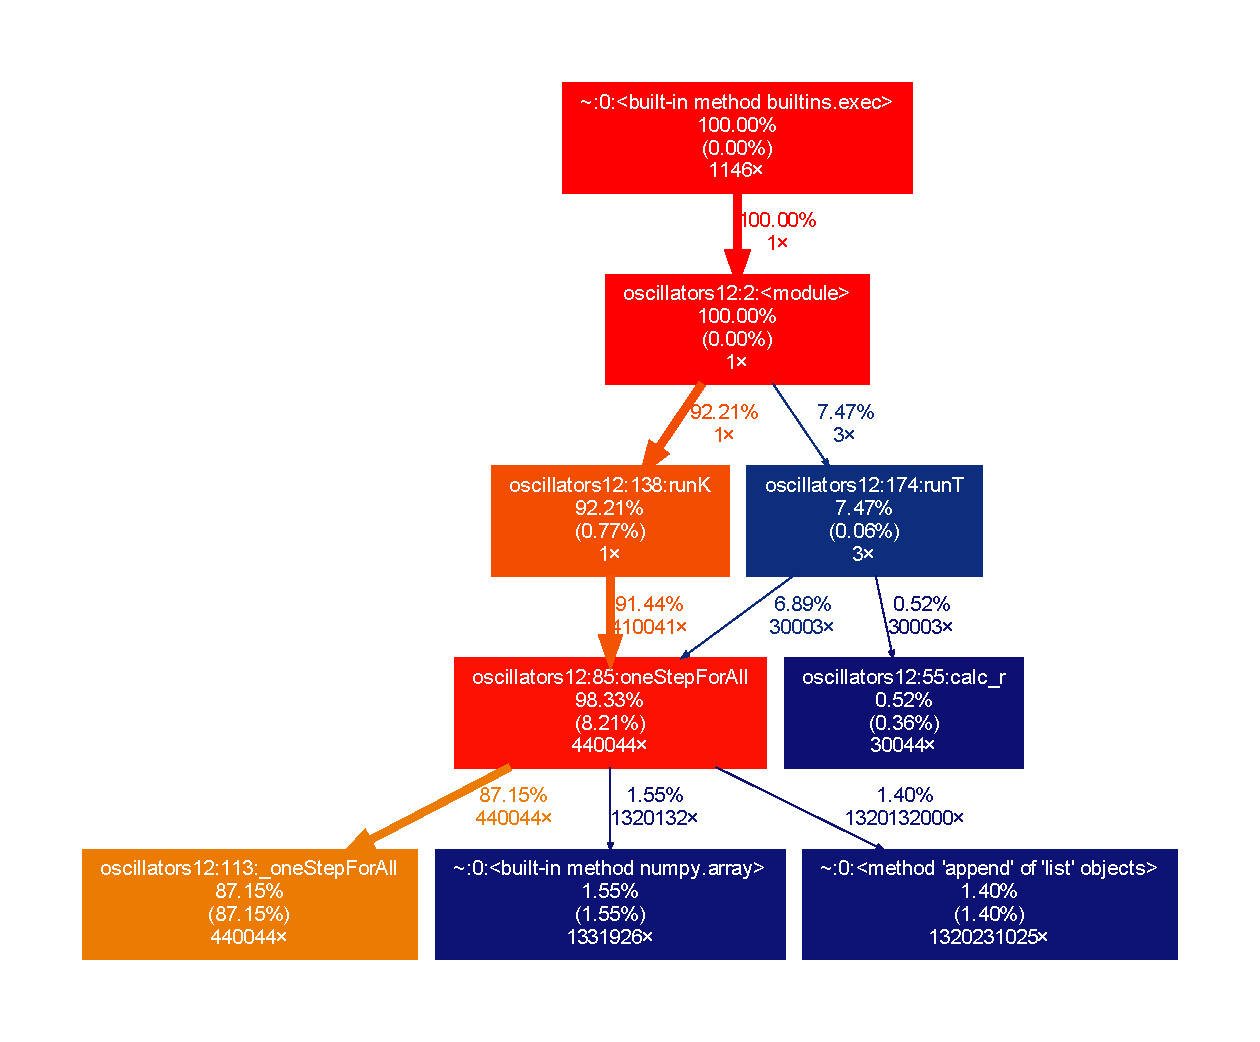
\includegraphics[width=\textwidth]{graphics/profile12.pdf}
	\caption{Profile of code for task 1 and 2}
	\label{profile12}
\end{figure}









\subsubsection{Numerical integration}
The strategy to integrate the consistency equation is to loop through different values of $r$ and check which ones make the right-hand side approximately equal to one. 
The precision of this approximation can be adjusted by changing the \code{rHysteresis} variable, which sets the acceptable range of values around 1 for the right-hand side of the consistency equation.
In a loop around this one, we cycle through the different values for K to get the values of the desired $r(K)$ relationship. 
The results are then graphed in figure \ref{1} together with the simulated points.




\subsubsection{Results}

\begin{figure}[H]
	\centering
	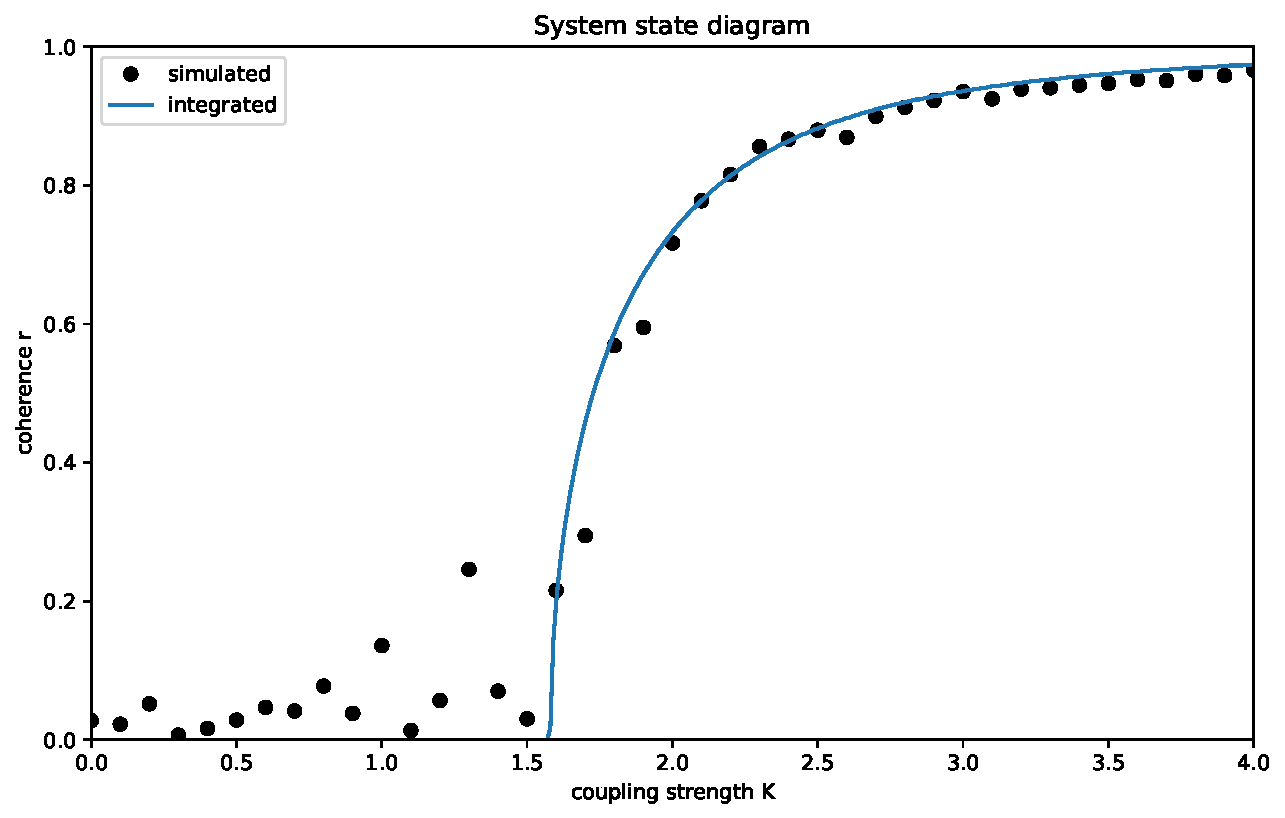
\includegraphics[width=0.8\textwidth]{graphics/1_K-vs-r_omegaDistr=normal_N=1000_1611577031.pdf}
	\caption{Diagram of limiting $r_\infty$ for different values of K}
	\label{1}
\end{figure}


The first observation is that 







%%%%%%%%%%%%%%%%%%%%%%%%%%%%%%%%%%%%%%%%%%%%%%%%%%%%%%%%%%%%%%%%%%%%%%%%%%%%%%%%%%%%%%%%%%%%%%%%%%%%%%%%%%%%%%%%%%%%%%%%%%%%%%%%%
\clearpage
\subsection{$r(t)$ for $K = [1, 2,3]$} \label{r(t)}

The simulation procedure for is the same as for \runK, with 2 exceptions:
\begin{enumerate}
	\item there is still $K$-loop (with limited values $K = [1,2,3]$), but there is no resetting of the population to new random values at the beginning of each such loop.
	\item $r(t)$ is now calculated at every (simulation!) time step $t$.
\end{enumerate}

The previous method of assigning new random values to the state variables of all oscillators did not work for some reason here. 
Instead, a bug occurred in which the final values of the last run were used as the starting values of a new run.%
	\footnote{My hypothesis is that this is about memory management in python. Sometimes during other assignment of variables or objects, it merely creates a pointer instead of copying the value into a separate location in memory.}
Therefore I had to go another way: now I recreate the \oscpop object anew in every loop. 

After that, \runT is executed, which calls \code{OscPopulation.calc\_r()} at every time step. 
\code{calc\_r()} calculates $r(t)$ in one of two different but equivalent ways. 
In one way, actual complex numbers are added up and divided by N. 
To get a value for $r$, the modulus of the resulting complex number is taken. 
$$ r_t = \lvert \sum_{n=0}^N e^{\theta^n_t \cdot i} \rvert$$
The other way is to compute the double sum of real and imaginary component of the complex number (using the $sin()$ and $cos()$ relationships after DeMoivre's and Euler's formula).
These two sums are also divided by N, yielding the average real and imaginary component of the \oscpop at this time. 
From there, $r$ can be calculated through a square root:
\begin{align*}
	realsum 	&= \sum_{n=0}^N \frac{\cos(\theta^n_t)}{N} \\
	imsum 		&= \sum_{n=0}^N \frac{\sin(\theta^n_t)}{N} \\
	r 			&= \sqrt{realsum^2 \cdot imsum^2}
\end{align*}
I tried both versions to double check the results and hoping one would give a performance boost over the other, but both have approximately the same speed.
In the end, \code{calc\_r()} returns a list of $r(t)$ which will be appended to a list-of-lists with the $r$ values for all chosen $K$. 
These different trajectories are once again graphed: figure \ref{2}.

\subsubsection{Results}

\begin{figure}[H]
	\centering
	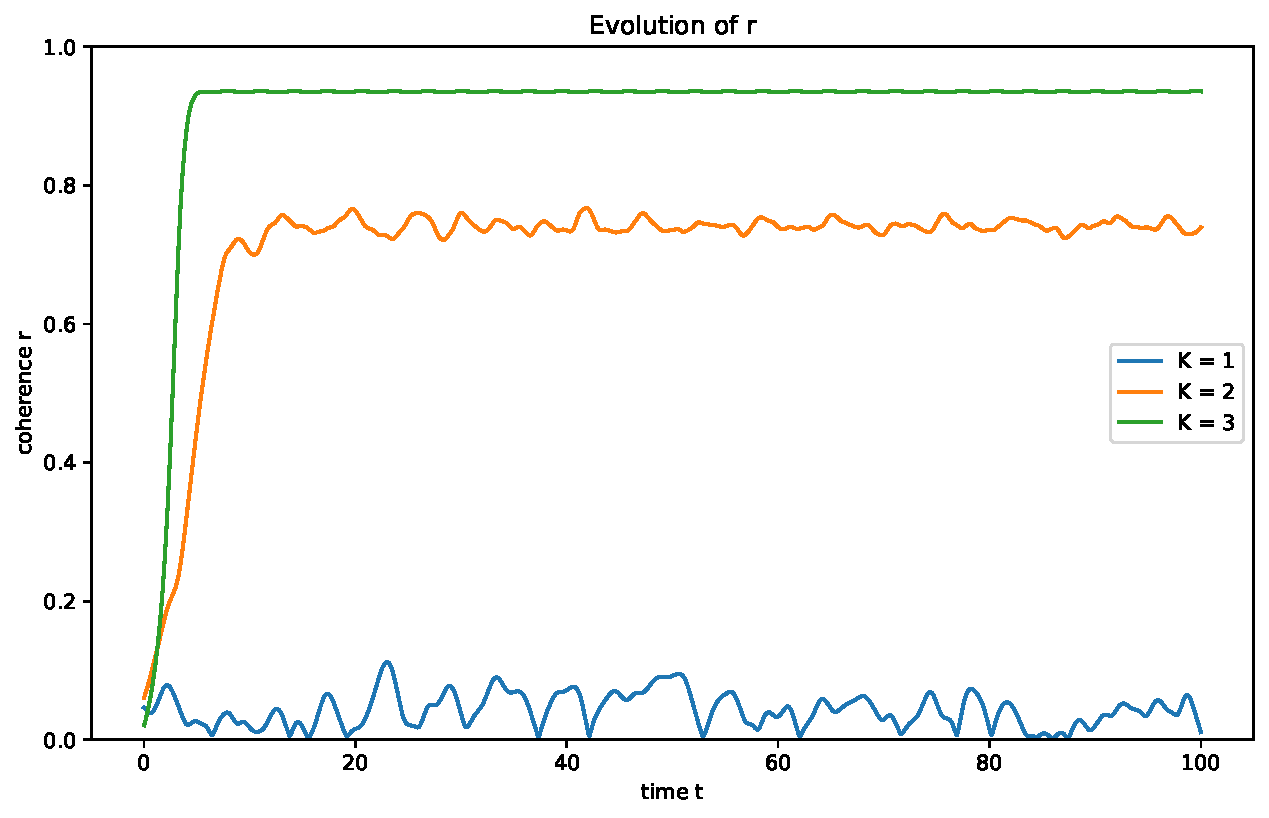
\includegraphics[width=0.8\textwidth]{graphics/2_t-vs-r_omegaDistr=normal_N=1000_1611577412.pdf}
	\caption{$r(t)$ over time for 3 different values of $K$}
	\label{2}
\end{figure}





















%%%%%%%%%%%%%%%%%%%%%%%%%%%%%%%%%%%%%%%%%%%%%%%%%%%%%%%%%%%%%%%%%%%%%%%%%%%%%%%%%%%%%%%%%%%%%%%%%%%%%%%%%%%%%%%%%%%%%%%%%%%%%%%%%
%%%%%%%%%%%%%%%%%%%%%%%%%%%%%%%%%%%%%%%%%%%%%%%%%%%%%%%%%%%%%%%%%%%%%%%%%%%%%%%%%%%%%%%%%%%%%%%%%%%%%%%%%%%%%%%%%%%%%%%%%%%%%%%%%
\clearpage
\FloatBarrier
\bigskip\noindent
{\Large\textbf{Omegas uniformly distributed}}
\addcontentsline{toc}{subsection}{\\\textbf{Omegas uniformly distributed}}
%%%%%%%%%%%%%%%%%%%%%%%%%%%%%%%%%%%%%%%%%%%%%%%%%%%%%%%%%%%%%%%%%%%%%%%%%%%%%%%%%%%%%%%%%%%%%%%%%%%%%%%%%%%%%%%%%%%%%%%%%%%%%%%%%
\subsection{$r_{\infty}(K)$}


\subsubsection{Program profile}
The profile of the code for tasks 3, 4 and 5 can be seen in figure \ref{profile345}.
\begin{landscape}
\begin{figure}[p]
	\centering
	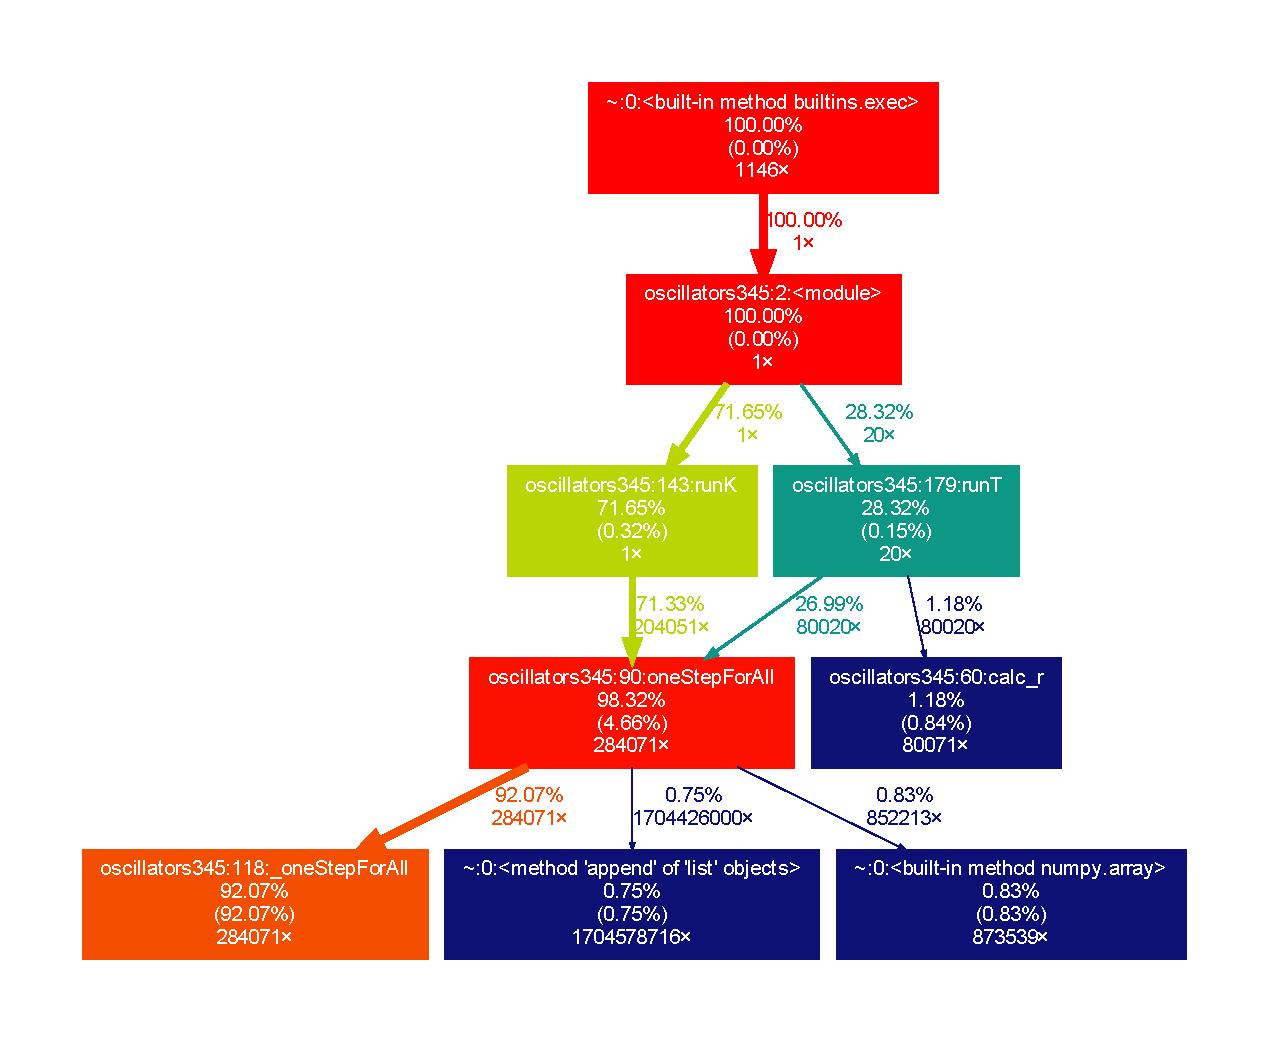
\includegraphics[width=26cm]{graphics/profile345.pdf} % can also use angle = 90
	\caption{Profile of code for task 3, 4 and 5}
	\label{profile345}
\end{figure}
\end{landscape}


\subsubsection{Results}

\begin{figure}[h]
	\centering
	\begin{subfigure}{0.8\textwidth}
		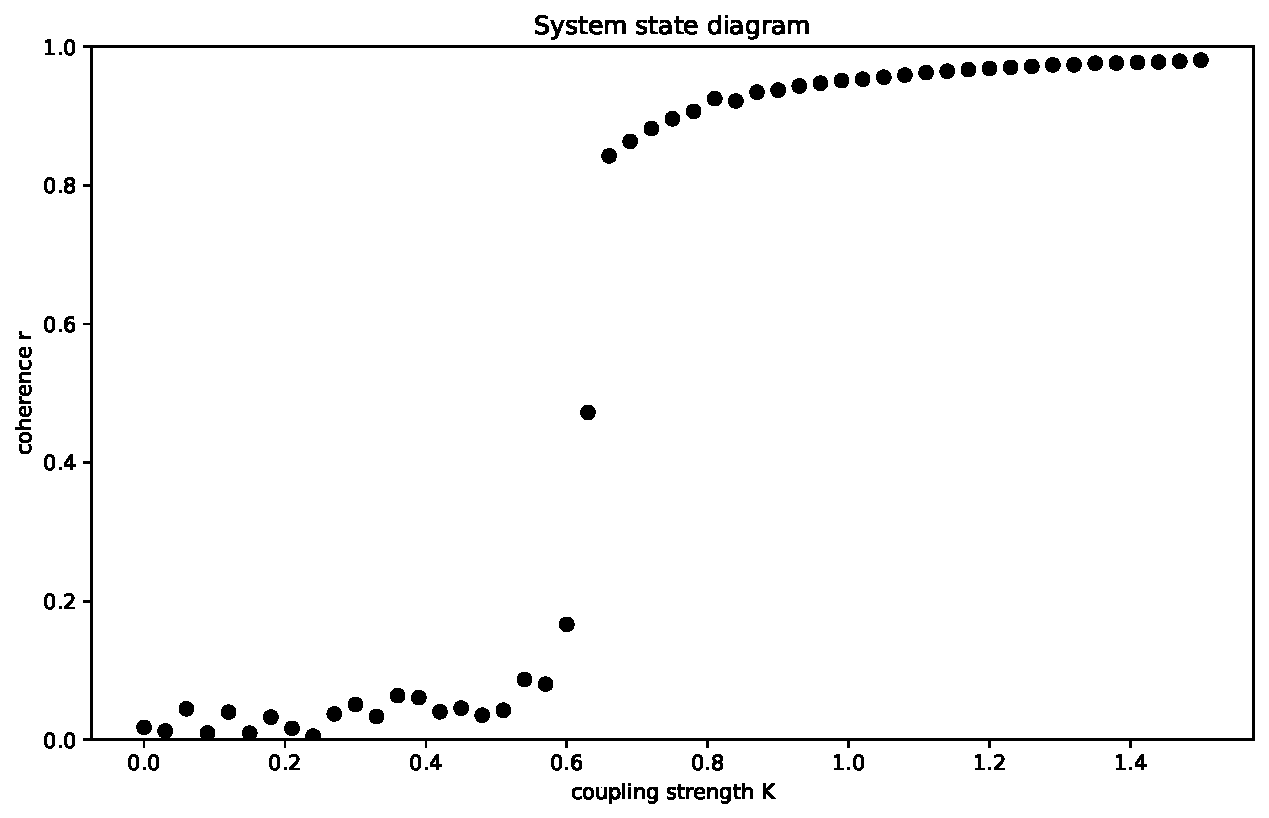
\includegraphics[width = \textwidth]{graphics/3_K-vs-r_omegaDistr=uniform_zoomed_N=2000_1611568972.pdf}
		\caption{zoomed in}
		\label{3zoomedin}
	\end{subfigure}
	\begin{subfigure}{0.8\textwidth}
		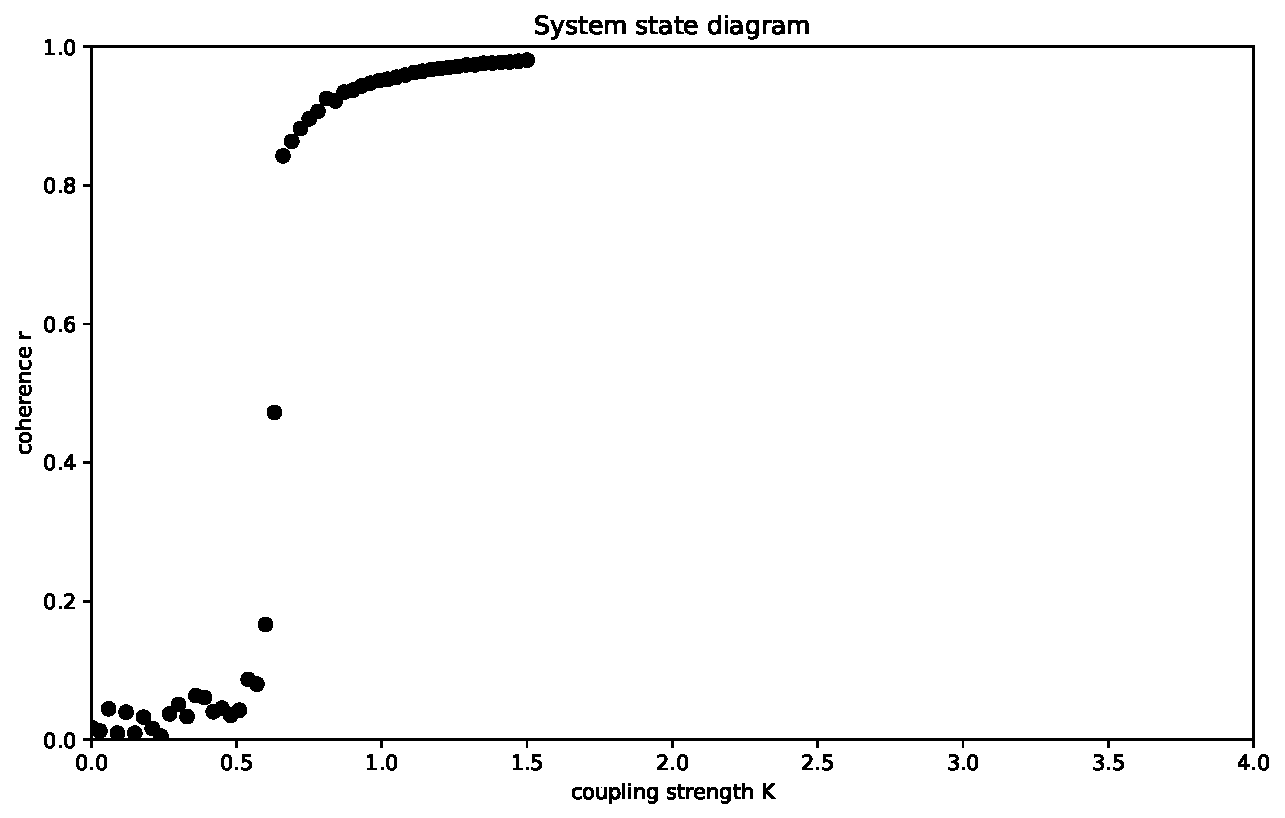
\includegraphics[width = \textwidth]{graphics/3_K-vs-r_omegaDistr=uniform_N=2000_1611568972.pdf}
		\label{3zoomedout}
		\caption{zoomed out, for better comparison with figure \ref{1}}
	\end{subfigure}
	\caption{$r_\infty(K)$ for different values of K, with a uniform distribution of $\omega$s}
	\label{3}
\end{figure}













%%%%%%%%%%%%%%%%%%%%%%%%%%%%%%%%%%%%%%%%%%%%%%%%%%%%%%%%%%%%%%%%%%%%%%%%%%%%%%%%%%%%%%%%%%%%%%%%%%%%%%%%%%%%%%%%%%%%%%%%%%%%%%%%%
\clearpage
\subsection{$r(t)$ for different initial conditions $\theta_0$}

To run simulations repeatedly while keeping selected initial conditions the same, I implemented the following. 
First, a 'reference' \oscpop object is initiated. 
Then a loop begins in which a 'temporary' \oscpop objects (newly initialised with entirely random values) is created. 
The desired initial conditions from the reference object are then written into the temporary object: here, the $\omega$s are kept, later the $\theta$s. 
\code{runT()} is executed on the temporary object and the returned trajectory saved into another list-of-lists. 








\subsubsection{Results}

\begin{figure}[h]
	\centering
	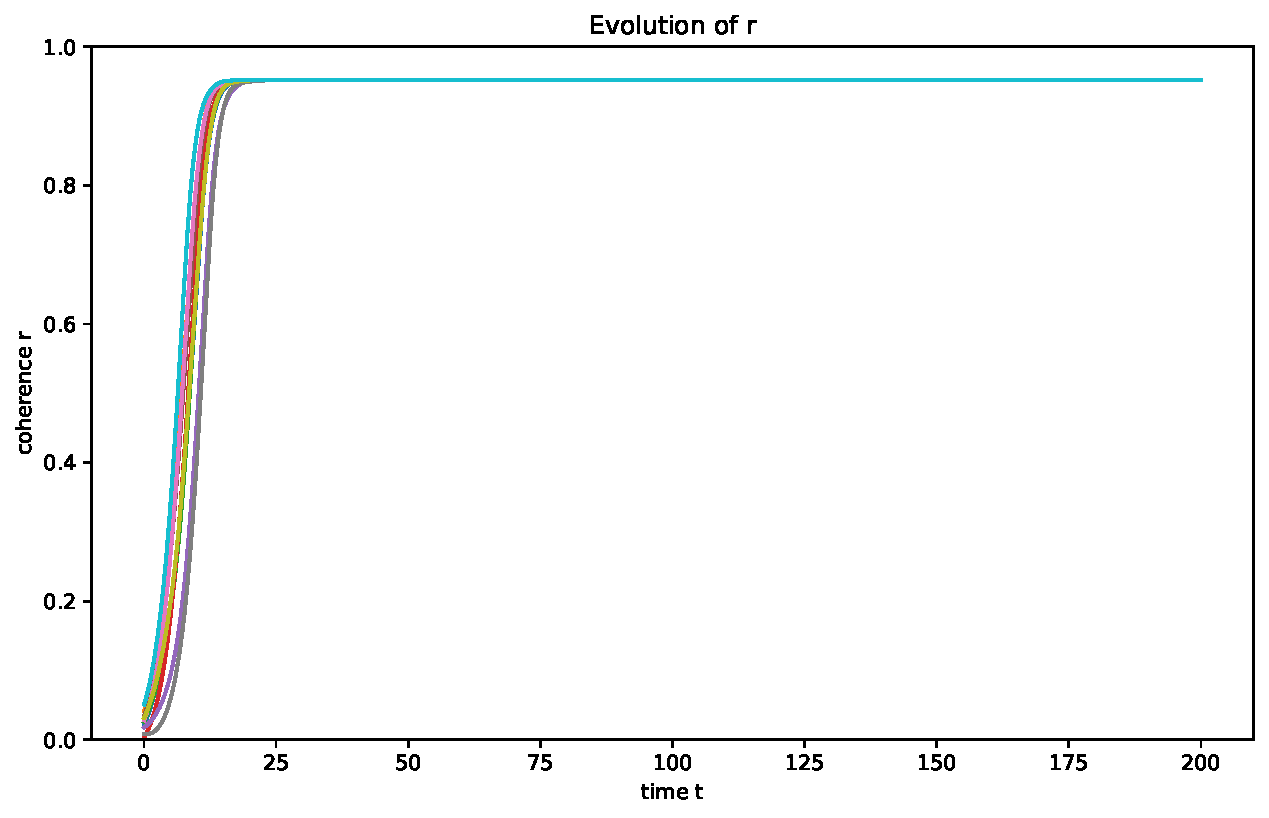
\includegraphics[width=0.8\textwidth]{graphics/4_t-vs-r_fixedOmegas_omegaDistr=uniform_N=2000_1611570486.pdf}
	\caption{$r(t)$ over time for 10 different initial conditions of $\theta$}
	\label{4}
\end{figure}











%%%%%%%%%%%%%%%%%%%%%%%%%%%%%%%%%%%%%%%%%%%%%%%%%%%%%%%%%%%%%%%%%%%%%%%%%%%%%%%%%%%%%%%%%%%%%%%%%%%%%%%%%%%%%%%%%%%%%%%%%%%%%%%%%
\clearpage
\subsection{$r(t)$ for different initial conditions $\omega_0$}






\subsubsection{Results}

\begin{figure}[h]
	\centering
	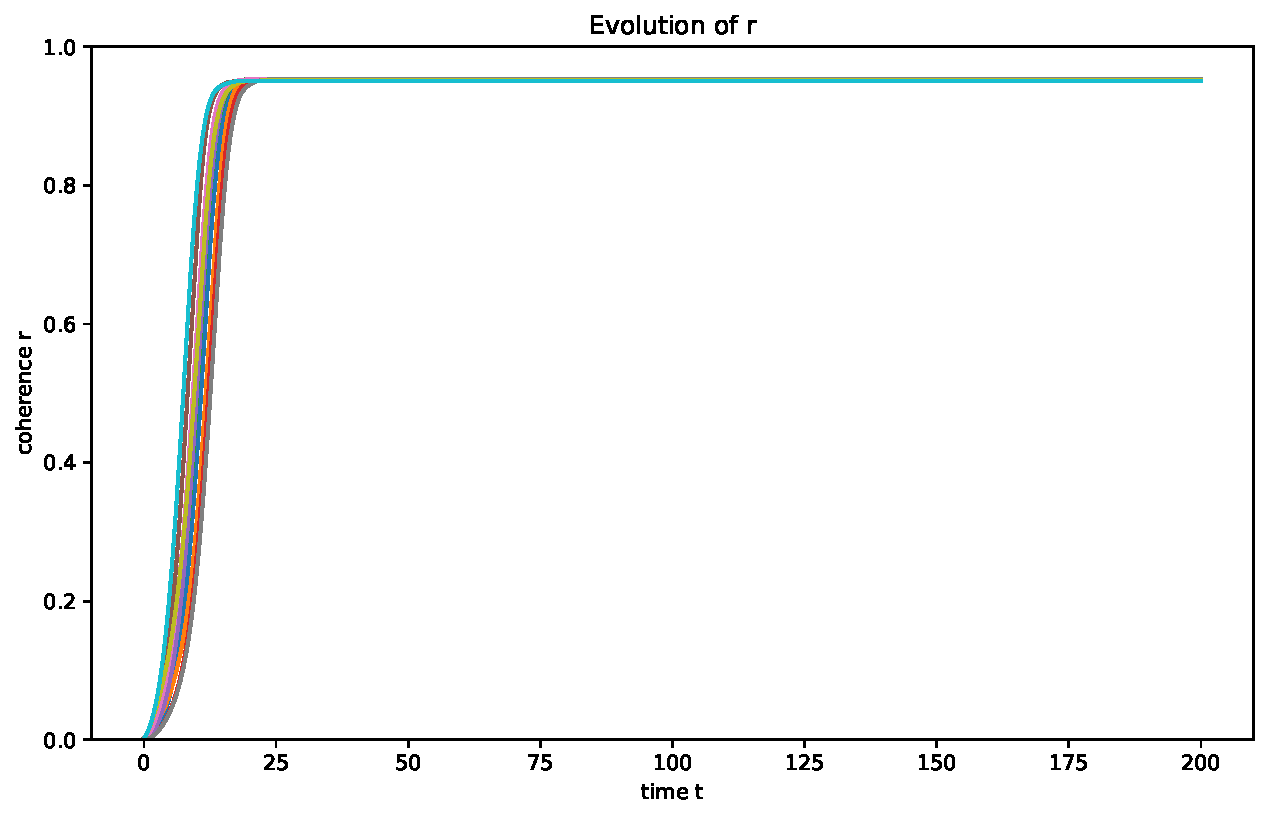
\includegraphics[width=0.8\textwidth]{graphics/5_t-vs-r_fixedThetas_omegaDistr=uniform_N=2000_1611572031.pdf}
	\caption{$r(t)$ over time for 10 different initial conditions of $\omega$}
	\label{5}
\end{figure}































\end{document}